\section{Technische Realisierung}

\subsection{Eingesetzte Entwurfsmuster}
\subsubsection{Mediator Pattern - Der Text Transfer Agent}
Neben der Verwaltung von klienten- und wohngruppenspezifischen Daten ist die Überführung von Textstücken aus verschiedenen Teilen des
Dokumentationsprogramms die Hauptfunktion der \EBP. Diese Funktion wird im folgenden \textit{Text Transfer} genannt. \newline
Der \textit{Text Transfer} soll aus den Masken Bewohner$\rightarrow$Protokoll, Bewohner$\rightarrow$Projekt und Wohngruppe$\rightarrow$Gruppenbuch
erfolgen. Gespeichert werden die Textfragmente in den verschiedenen Feldern der Betreuungsplanung eines beliebigen Bewohners. Die Unterschiedlichkeit
der Quellen für die zu transferierende Textfragmente und die Variation an Zielfelder war die Schwierigkeit bei der Implementierung dieser
Funktionalität. Da die Anzahl an Objekten, die als Quelle dienen, im Programmverlauf stark variieren kann, muss der Lösungsansatz sehr flexibel
implementiert sein. Abbildung \ref{unstrukturiert} zeigt die Vielzahl an möglichen Kommunikationswegen zwischen den einzelnen Objekten.\\
\begin{figure*}[htp]
	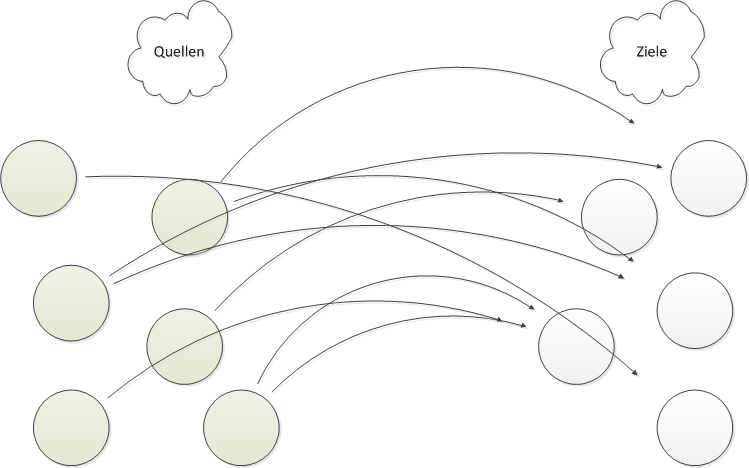
\includegraphics[width=0.8\textwidth]{unmediated}
	\caption{Kommunikationswege zwischen den Objekten}
	\label{unstrukturiert}
\end{figure*}
Um nicht jeden Kommunikationsweg einzeln verwalten zu müssen, wurde der \textit{Text Transfer} in Form des Mediator Patterns entworfen. Den Zweck
eines Mediators definiert GAMMA wie folgt: \\
``Definiert ein Objekt, welches das Zusammenspiel einer Menge von Objekten in sich kapselt. Vermittler fördern lose Kopplung, indem sie Objekte davon
abhalten, aufeinander explizit Bezug zu nehmen. Sie ermöglichen es Ihnen, das Zusammenspiel der Objekte von ihnen unabhängig zu
variieren \cite[S. 385]{Entwurfsmuster}.''\\
Auf einen abstrakten Mediator wird hier verzichtet 

\begin{figure*}[htp]
	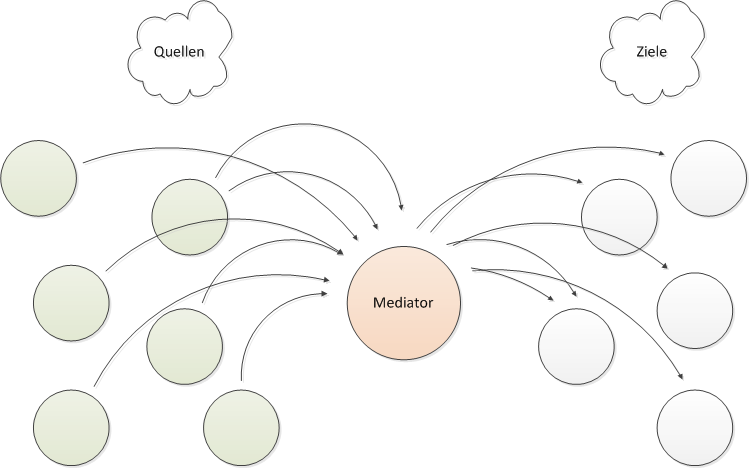
\includegraphics[width=0.8\textwidth]{mediated}
	\caption{Kommunikationswege zwischen den Objekten, koordiniert durch einen Mediator}
	\label{unstrukturiert}
\end{figure*}
\subsubsection{Observer Pattern - Signal Slot Konzept}
\subsubsection{Model View Controller Pattern - Datenvisualisierung}

\subsection{Architektur}
\subsubsection{Aufteilung der Module}
\subsubsection{Buildsystem}

\subsection{Qt als Grafikbibliothek}

\subsection{Persistenzschicht mit ODB (libEBPdb)}
\subsubsection{Object-Relational-Mapping (ORM)}
Um die Daten einer relationellen Datenbank auf Objekte innerhalb einer Programmiersprache abzubilden gibt es prinzipiell zwei Ansätze.
Entweder wird der Code der die Eigenschaften eines Objekts aus der Datenbank liest und schreibt manuell implementiert, oder aber es wird ein 
Mechanismus eingesetzt, der automatisiert Variablen eines Objekts den Feldern einer Datenbank zuordnet.
\subsubsection{Datenbankunabhängigkeit}
\subsubsection{Code-Generierung}
\subsubsection{Integration in das Buildsystem}
\subsubsection{Datenbankschema}
\subsubsection{Abstraktion der Schnittstelle}
